\documentclass[sigconf,review]{acmart}



%% Copyright information
\setcopyright{acmcopyright} % TODO: copyright?
\copyrightyear{2022}
\acmYear{2022}
\acmDOI{10.1145/1122445.1122456} % TODO: DOI?

%% These commands are for a PROCEEDINGS abstract or paper.
\acmConference[Pittsburgh '22]{Pittsburgh '22: NIER - New Ideas and Emerging Results (ICSE 2022)}{May 21--29, 2022}{Pittsburgh, PA, USA}
\acmBooktitle{Pittsburgh '22: NIER - New Ideas and Emerging Results (ICSE 2022), May 21--29, 2022, Pittsburgh, PA, USA}
\acmISBN{978-1-4503-XXXX-X/18/06} % TODO: ISBN

%% Packages

% \usepackage[paperwidth=8.50in, paperheight=11in]{geometry} %% option clash
\usepackage[T1]{fontenc}
%\usepackage[latin1]{inputenc}

% \usepackage[protrusion=true,expansion=true]{microtype} %% option clash

% for inline lists
\usepackage[inline]{enumitem}
% for nice internal links
\usepackage{hyperref}

\begin{document}

\title{A Sustainable Approach to Developing Software in Well Understood Domains}

\author{Jacques Carette}
\orcid{0000-0001-8993-9804}
\affiliation{
  \department{Computing and Software}
  \streetaddress{1280 Main Street West}
  \institution{McMaster University}
  \city{Hamilton}
  \state{Ontario}
  \postcode{L8S 4L8}
  \country{Canada}}
\email{carette@mcmaster.ca}

\author{Spencer Smith}
\orcid{0000-0002-0760-0987}
\affiliation{
  \department{Computing and Software}
  \streetaddress{1280 Main Street West}
  \institution{McMaster University}
  \city{Hamilton}
  \state{Ontario}
  \postcode{L8S 4L8}
  \country{Canada}}
\email{smiths@mcmaster.ca}

\begin{abstract}
  Missing abstract. % TODO: abstract
\end{abstract}


%       Generator:   http://dl.acm.org/ccs.cfm
% TODO: This is a temporary CCSXML and \ccsdesc list
\begin{CCSXML}
<ccs2012>
   <concept>
       <concept_id>10003752.10003753.10010622</concept_id>
       <concept_desc>Theory of computation~Abstract machines</concept_desc>
       <concept_significance>500</concept_significance>
       </concept>
   <concept>
       <concept_id>10011007.10011006.10011066.10011070</concept_id>
       <concept_desc>Software and its engineering~Application specific development environments</concept_desc>
       <concept_significance>300</concept_significance>
       </concept>
   <concept>
       <concept_id>10011007.10011074.10011075.10011076</concept_id>
       <concept_desc>Software and its engineering~Requirements analysis</concept_desc>
       <concept_significance>300</concept_significance>
       </concept>
   <concept>
       <concept_id>10011007.10011006.10011060.10011690</concept_id>
       <concept_desc>Software and its engineering~Specification languages</concept_desc>
       <concept_significance>300</concept_significance>
       </concept>
   <concept>
       <concept_id>10011007.10011074.10011092.10011782</concept_id>
       <concept_desc>Software and its engineering~Automatic programming</concept_desc>
       <concept_significance>500</concept_significance>
       </concept>
 </ccs2012>
\end{CCSXML}

\ccsdesc[500]{Theory of computation~Abstract machines}
\ccsdesc[300]{Software and its engineering~Application specific development environments}
\ccsdesc[300]{Software and its engineering~Requirements analysis}
\ccsdesc[300]{Software and its engineering~Specification languages}
\ccsdesc[500]{Software and its engineering~Automatic programming}
%% End of generated code

\keywords{code generation, document generation, knowledge capture,
  software engineering, scientific software}

% set up math environment
\newtheorem{defn}{Definition}

\maketitle

\section{Introduction} \label{ch:introduction}
% What if we're doing it all wrong?

``Software'' is not uniform. To use the exact same process for
developing an embedded safety-critical piece of code (like that of
a pacemaker), the flight control software for an airplane, a one-off
script for moving some files around, and some amusing animations on
one's personal web site, is patently ridiculous.

The same is true in say, civil engineering: you don't need architects,
licensed engineers and a million permits to build a small shed in your
backyard, but you do need them to build a $100$ story skyscraper.

Which brings us to our central topic: there are some kinds of software
where our current development methods \emph{are all wrong}. Our task
is to define exactly which type of software we have in mind, and then
derive an entirely different development methodology that is
customized to the special characteristics of that strict subset.

There are many properties of software that can be used for providing
a classification. Here we will focus on one particular ``axis'': how
\textbf{well understood} it is. The majority of the next section will
be devoted to explaining exactly what this means. Once that is set up,
we can then unravel some operational consequences: how the characteristics of
well understood softare lead to innovative methods of building such
software. As this might be perceived as too abstract, we give a very
concrete example. Of course, our ideas do not exist in a vacuum: we were
inspired by a number of connected ideas, and we then give credit where
credit is due. More than just ideas, there are also technologies that back
these ideas, some of which we're already using, others which lie in our
future, and we outline some of these as well. %add references to the section numbers?

\section{What is ``well understood'' Software?}\label{ch:wellUnderstood}

\begin{defn}
A software domain is \emph{well understood} if
\begin{enumerate}
\item the domain knowledge (DK) is codified,
\item the computational interpretation of the DK is clear,
\item the engineering of code to perform said computations is well
understood.
\end{enumerate}
\end{defn}

By \emph{codified}, we mean that the knowledge exists in standard form in
a variety of textbooks. For example, many domains of knowledge in engineering
use differential equations as models. Furthermore, the quantities of interest
are known, given standard names and standard units. In other words, there is
an established vocabulary and body of knowledge that is uncontroversial.

We can further refine these high level ideas as follows, where we use
the same numbering as above to indicate which part of the definition is
being directly refined, but where the refinement nevertheless should be
understood more holistically.
\begin{enumerate}
\item Models in the DK \emph{can be} written formally.
\item Models in the DK \emph{can be} turned into functional relations by
 existing mathematical steps.
\item Turning these functional relations into code is also an understood
 transformation.
\end{enumerate}
Perhaps the most important aspect of this refinement is that the last two
parts deeply involve \emph{choices}: What quantities are considered inputs,
outputs and parameters to make the model functional? There are also a host
of choices, including which programming language, but also software
architecture, data-structures, algorithms, etc, which are also part of
creating the code.

It is important to understand that \emph{well understood} does not imply
\emph{choice free}.  Writing a small script to move some files around can
be easily written as a Shell script, or in Python or in Haskell, depending on
the author's style. In all cases, assuming the author chooses a language
in which they are fluent, the job will be entirely straightforward.

Lest our reader gets misled into thinking that code is the only artifact
that matters, we should explicitly refine our definition in a different
direction, equally important.
\begin{enumerate}
\item The meaning of the models is understood at a human-pedagogical
level, i.e. it is explainable.
\item Combining models is also explainable. Thus the \emph{transformers}
  we mentioned before %this is actually the first time transformers are mentioned
  simultaneously operate on mathematical representations
and on explanations. This requires that English descriptions also be
captured in the same manner as the formal-mathematical knowledge.
\item Similarly, the \emph{transformers} the arise from making software
oriented decisions requires that they be captured with a similar mechanism,
including English explanations as well.
\end{enumerate}

We dub these \emph{triform theories}, as a nod to \emph{biform theories}%
\cite{Farmer}. The idea is that we couple 
\begin{enumerate*}
\item an axiomatic description,
\item a computational description, and
\item an English description
\end{enumerate*}
of a concept.

It is important to notice that there are various kinds of choices
embedded in the different kinds of knowledge. They can show up simply as
\emph{parameters}, for example the gravity constant associated to a planet.
This also shows up as different transformers, for example turning
$F - m\cdot a = 0$ into $F\left(m, a\right) = m\cdot a$, i.e. from a 
conservation law into a computation. Note that, for motion computation, that
same conservation law is often rewritten as $a\left(m,F\right) = F/m$ as
part of solving $a = \ddot{x}$ to obtain a position ($x$) as a function of time ($t$).
And we also get choices of phrasing, which are equivalent but may be more
adequate in context, for example.

\section{How would you go building that?}\label{ch:process}

So what would be a reasonable process for building a piece of software
assuming some kind of infrastructure exists for recording the kind of
knowledge outlined in~\autoref{ch:wellUnderstood}? Let us outline a
chronological ``story'' of such an idealized process.  It is important to
note that we're \textbf{not} outlining the process to follow, but rather
the \emph{idealized process} (influenced by Parnas' \cite{Parnas1986}).

\begin{enumerate}
\item\label{it:problem} Have a problem to solve, or task to achieve, which
falls into the realm where \emph{software} is likely to be the central part of
the solution.
\item\label{it:understood} Convince oneself that the underlying problem domain
is \emph{well understood}, as defined in~\autoref{ch:wellUnderstood}.
\item\label{it:probdesc} Describe the problem:
  \begin{enumerate}
  \item Find the base knowledge (theory) in the pre-existing library
    or, failing that, write it if it does not yet exist,
  \item Assemble the ingredients into a coherent narrative,
  \item Describe the characteristics of a good solution,
  \item Come up with basic examples (to test correctness, intuitions, etc).
  \item Identify the naturally occurring known quantities associated to the
    problem domain, as well as some desired quantities. For example,
    some problems naturally involve lengths lying in particular
    ranges, while others will involve ingredient concentrations, again
    in particular ranges.
  \end{enumerate}
\item\label{it:refine} Describe, by successive transformations, how the natural
knowledge can be turned from a set of relations (and constraints) into a
deterministic\footnote{For the moment, we explicitly restrict our domain to
deterministic solutions, as a meta-design choice. This can be expanded later.}
input-output process.
  \begin{enumerate}
  \item This set of relations might require \emph{specializing} the
    theory (eg. from $n$-dimensional to $2$-dimensional, assuming no
    friction, etc).  These \emph{choices} need to be documented, and are
    a crucial aspect of the solution process. The \emph{rationale} for the
    choices should also be documented. Lastly, whether these choices are
    likely or unlikely to change in the future should be recorded.
  \item This set of choices is likely dependent, and thus somewhat ordered.
  In other words, some \emph{decisions} will enable other choices to be
  made that would otherwise be unavailable. Eg: some data involved in the
  solution process is orderable, so that sorting is now a possibility that
  may be useful.
  \end{enumerate}
\item\label{it:tocode} Describe how the computation process from step
\ref{it:refine} can be turned into code. Note that the same kinds of choice
can occur here.
\item\label{it:recipe} Turn the steps (i.e.\ from items~\ref{it:refine} and
\ref{it:tocode}) into a \emph{recipe}, aka program, that weaves together
all the information into a variety of artifacts (softifacts). These can
be read, or execute, or \ldots\ as appropriate.
\end{enumerate}

While this last step might appear somewhat magical, it isn't. The whole
point of defining \emph{well understood} is to enable that last step. A
suitable knowledge encoding is needed to enable it, but this step is a
reflection of what humans currently themselves do when assembling these very
same softifacts. We are merely being explicit about how to go about
mechanizing these steps.

What is missing is an explicit \emph{information architecture} of each of
the necessary softifacts. In other words, what information is necessary to
enable the mechanized generation of each softifact? It turns out that many
of them are quite straightforward.

It is worthwhile to note that way too many research projects skip
step~\ref{it:problem} and~\ref{it:probdesc}: in other words, they never really
write down what problem they're trying to solve. This is part of the
\textbf{tacit knowledge} of a lot of research software.  It is crucial to our
whole process that this knowledge go from tacit to explicit. This is also one
of the fundamental recognitions of \emph{Knowledge
Management}~\cite{KM-textbook}.

TODO: insert graphical illustration of the funnel from information to
softifacts.

\begin{figure*}[h]
  \centering
  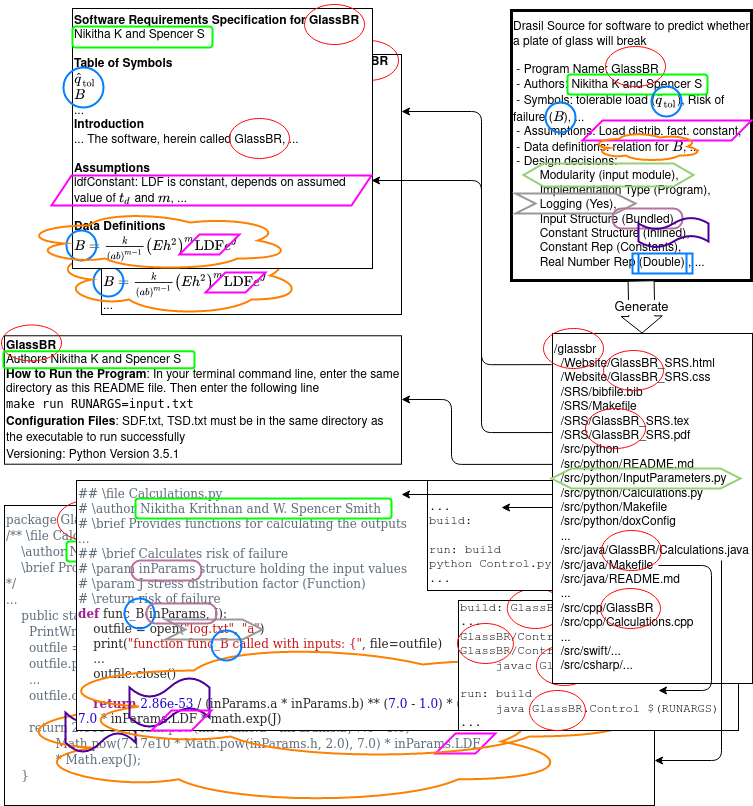
\includegraphics[width=\linewidth]{assets/DrasilSupportsChange-right-portrait-overlapped-ungrouped-v1.drawio.png}
  \caption{TODO: caption}
  \Description{TODO: description}
\end{figure*}

\section{Example}\label{ch:example}

\section{Connected Ideas}\label{ch:ideas}

A multitude of ideas, old and new, have influenced us. They appear
indirectly in our work; we use the conceptual aspects, and not the
associated technologies (when they exist). The technologies we do use
are in Section~\ref{ch:techniques}.

We do not always use the original conceptualization of the work, but
a modern re-interpretation, incorporation various ``lessons learned''
through years of use. To keep things short, we outline our take-away, and refer
the reader to the original literature for the initial view of the ideas.

\section{Re-organizing artifacts}

The most important idea that got all of this started is
\emph{literate programming}\cite{Knuth1984}. A key observation here
is that computer code really has two audiences: the computer, proxied
via a compiler or interpreter, and human readers. Traditionally, code
is arranged for the convenience of the compiler\footnote{we use ``compiler''
even though this applies equally well to interpreters}. Many languages
are quite inflexible with respect to how code must be arranged to be
acceptable. This directly clashes with the desire to inform the
human reader of the code as to the \emph{underlying story} that forms the
backbone of why the code is written the way it is.

Thus the fundamental ideas of literate programming are:
\begin{enumerate}
\item The idea of not writing the eventual artifacts directly,
\item Of being able to ``chunk up'' pieces of code in arbitrary
ways,
\item Of writing a program to explicitly weave together the chunks
into a final program.
\end{enumerate}
In the end, two artifacts are generated: a human-readable ``story'' that
is nicely typeset, that follows a logical flow amenable to human understanding,
and a piece of code.

Not all literate programming tools actually support all these features.
For example \emph{literate Haskell} only keeps the feature of nice typesetting,
completely dropping the $3$ main ideas above!

The next source of idea is \emph{org-mode}\cite{org-mode}. A shallow view
is that org-mode is an Emacs major mode for plain text markup%
\footnote{taken literally from \url{https://orgmode.org}.}
\emph{and much more}.  It is that ``and much more'' which is of interest
here. Amongst other features, Org-mode lets you write documents that mixes many
different languages together. It also allows you to run certain code blocks
and insert their results into the document itself. And, like literate
programming, it also allows the export of both nice documents
(via \LaTeX) and code (via a tangling process). The paper
\textit{A Computing Environment for Literate Programming and
Reproducible Research}\cite{SchulteEtAl2012} further describes the features
and process. The possibilities are quite extensive.

A slightly different take on similar ideas is offered by
\emph{Jupyter notebooks} and 
\emph{JupyterLab}\footnote{\url{https://jupyter.org}}. To quote the
developers' own descriptions:

\begin{quote}
The Jupyter Notebook is an open-source web application that allows you to
create and share documents that contain live code, equations, visualizations
and narrative text. Uses include: data cleaning and transformation, numerical
simulation, statistical modeling, data visualization, machine learning, and
much more.
\end{quote}
\noindent and
\begin{quote}
JupyterLab is a web-based interactive development environment for Jupyter
notebooks, code, and data. JupyterLab is flexible: configure and arrange the
user interface to support a wide range of workflows in data science, scientific
computing, and machine learning. JupyterLab is extensible and modular: write
plugins that add new components and integrate with existing ones.
\end{quote}
The principal difference is that the main interface is a web page
which is furthermore \emph{very interactive}. It is also multi-lingual.
The weaving and tangling features, while somewhat present, are de-emphasized
over interactivity. The all-in-one interactive document is the most
important element.  The feature set is very appealing, and contributes greatly
to its success.

\paragraph{Commentary:} The main weakness in all of these approaches is
that they are all centered on a single-document idea. The information
contained in the document itself is not re-usable. So while all three
ideas are a definite improvement over more traditional means of doing
development, it is still not enough. Furthermore, all three approaches
still involve hand-writing a lot of code, even though that code is
somewhat liberated from the strictures imposed by the languages themselves.

\section{The rest}
\begin{itemize}
\item cognitive work analysis, ecological interface design
\item knowledge management
\item ontologies, domain knowledge
\item biform theories
\item variabilities and commonalities, program families,
software product lines.
\item re-use
\item views (software architecture)
\item software artifacts
\item (re)certification
\item some ities: traceability, consistency
\item reproducible research
\item knowledge-based SE?
\item MDD, MDE
\item Grounded Theory
\end{itemize}

\section{Some Useful Technologies}\label{ch:techniques}

% first, some pointform notes, which will later be filled-in

\begin{itemize}
\item DSLs
\item code generation
\item program families
\item grammatical framework
\item plate, multiplate, optics
\item Problem Solving Environments (PSEs).

Another item to consider adding to the list is Problem Solving Environments
(PSE). A PSE is "[a] system that provides all the computational facilities
necessary to solve a target class of problems. It uses the language of the
target class and users need not have specialized knowledge of the underlying
hardware or software" ( Kawata et al., 2012 ). 
(From
\url{https://www.igi-global.com/dictionary/computer-assisted-problem-solving-environment-pse/41954}).
This is a different way to solve the same problem we are trying to solve. They
want the user to work with their domain knowledge, but they accomplish this (as
far as I can tell) by providing powerful general purpose tools and a language
to interface with these tools. They are focusing on run-time variability, while
we can focus on build time variability. An argument could be made that general
purpose tools are overwhelming for people. Being able to generate an
application that is as complex as the user needs, but no more complex, sounds
like a good thing to me. I believe they try to handle the complexity by
often providing a graphical DSL.

The idea of PSEs might be getting old. My quick search didn't find many newer
papers. This review article from 2010 might be useful:

\url{https://www.researchgate.net/publication/220147479_Review_of_PSE_Problem_Solving_Environment_Study}
  
\end{itemize}

%% Bibliography
\bibliographystyle{ACM-Reference-Format}
\bibliography{References}

\end{document}

% Good quotes:
% \begin{itemize}
% \item metaprograms are just programs
% \item models outside an integrated toolchain are insufficiently useful
% \end{itemize}
